%% Tex spellcheck = fr_FR
\chapter{Chapter 6 : Experimentations}

This final chapter will describe the different experimentations that were conducted. Two of those are simple GPS readings with a commercial GPS receiver and with an \gls{sdr}. The last one will be a spoofing attack on the commercial receiver.

\section{Equipement used}

\subsection{USRP B200 SDR}
There is a multitude of possible \gls{sdr} to chose from with different capabilities. We need one capable of transmitting and receiving on the GPS L1 frequency, this means the device needs to be able to transmit at 1575.42 MHz with a bandwidth of at least 30 Mhz.

We had one with these capabilities at the lab, the USRP B200. The device characteristics are as follows:
\begin{itemize}
	\item Frequency range: 70 MHz - 6 GHz
	\item Bandwidth: 56 MHz
	\item Sample rate: 61.44 MS/s
	\item USB 3.0 interface
\end{itemize}

\begin{figure}[H]
	\centering
	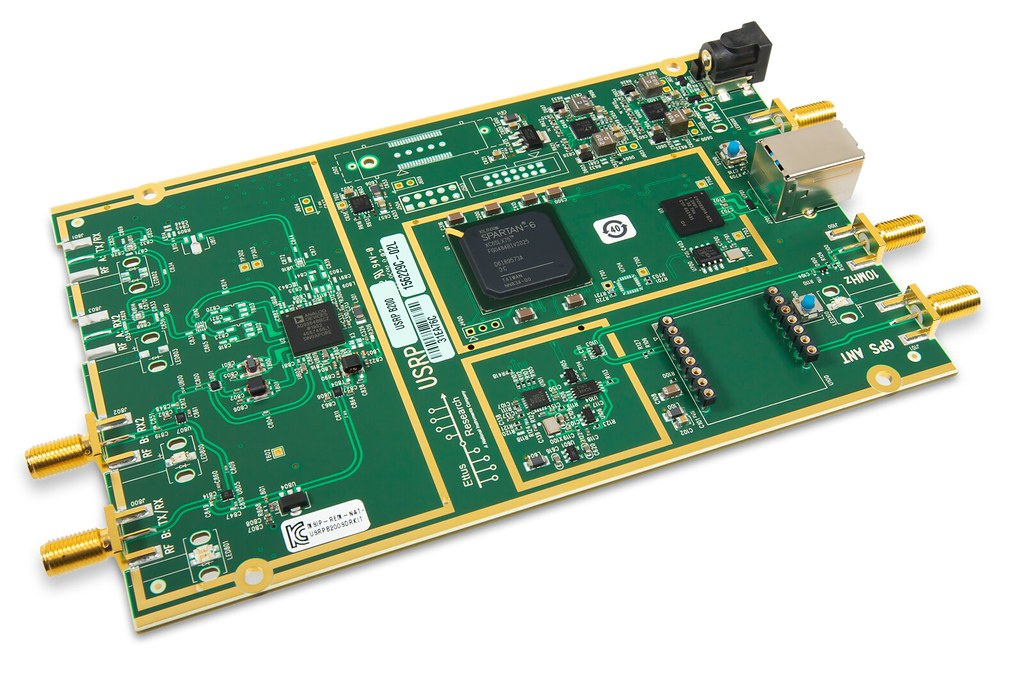
\includegraphics[width=0.8\linewidth]{usrp.jpg}
	\caption[USRP B200 without a case]{USRP B200 without a case Source: shop.trenz-electronic.de ref: URL18}
	\label{fig:usrp}
\end{figure}

\subsection{UBLOX Max-M10s - Commercial GPS receiver}

In order to test on hardware as close to a real-world, we tried to chose a \gls{gps} receiver as close as possible to the one used in the drone from the Windshape Paper \footcite{catry_development_2022}.
We needed a development board with the same chip and an SMA connector instead of an on board antenna, in order to connect the receiver directly to the \gls{sdr}. The drone used in the paper is a Parrot Anafi, which uses a UBLOX UBX-M8030. We couldn't find the exact model as a development board but we found the UBLOX Max-M10s which is relativly close to the UBX-M8030 and has a development board with an SMA connector: The SparkFun GPS-18037 \footcite{noauthor_gps-18037_nodate}.

\begin{figure}[H]
	\centering
	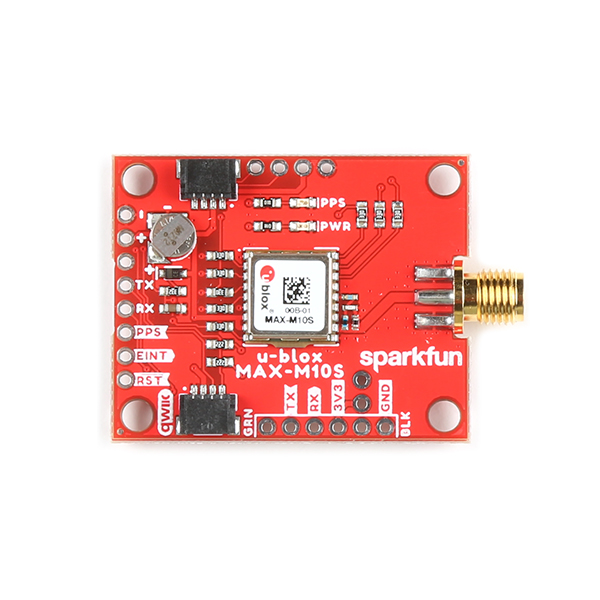
\includegraphics[width=0.8\linewidth]{gps_dev.jpg}
	\caption[MAX M10s Dev board]{MAX M10s Dev board Source: https://www.mouser.ch ref: URL19}
	\label{fig:gps_dev}
\end{figure}

\subsection{Antennas}

We used two different antennas for the experimentations. The first one is active and specific to GPS frequency\footcite{noauthor_ant-gps-sh2-sma_nodate} , the other one is a simple retractable antenna. We're testing these two antennas to assess the need for an active GPS antenna. Note that the active antenna has some filtering and amplification circuitry to improve the signal quality but need a power source to operate, this means that we need an external bias tee, powered by direct current source.

\begin{figure}[H]
	\centering
	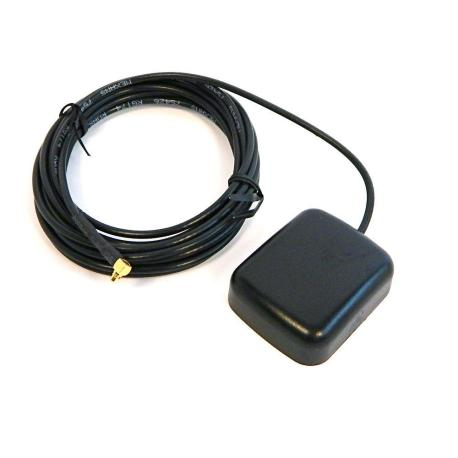
\includegraphics[width=0.8\linewidth]{active_antenna.jpg}
	\caption[Active GPS antenna]{Active GPS antenna Source: https://www.swiss-green.ch ref: URL20}
	\label{fig:active_antenna}
\end{figure}

\begin{figure}[H]
	\centering
	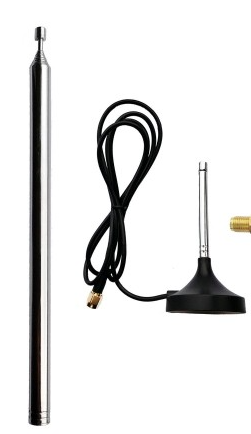
\includegraphics[width=0.4\linewidth]{passive_antenna.png}
	\caption[Passive retractable antenna]{Passive retractable antenna Source: www.passion-radio.com ref: URL21}
	\label{fig:passive_antenna}
\end{figure}

\begin{figure}[H]
	\centering
	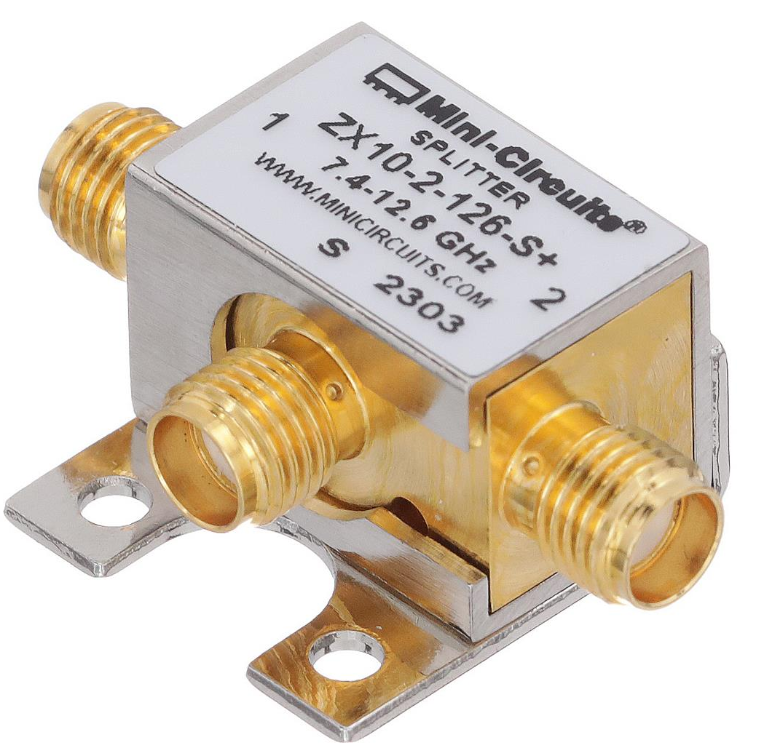
\includegraphics[width=0.6\linewidth]{bias_tee.png}
	\caption[Bias tee]{Bias tee to power the active antenna Source: www.artisantg.com ref: URL22}
	\label{fig:bias}
\end{figure}

\section{Softwares used}

The advantage of using an \gls{sdr} is the possibility to use a wide range of softwares to generate or receive signals.
In order to get a position fix with the \gls{sdr}, we used the GNURadio Companion \footcite{noauthor_gnu_nodate} to try to record raw data and get a position, we also used the GNSS SDR software \footcite{fernandez-prades_gnss-sdr_2024}  to read actual position directly with the \gls{sdr} as a frontend.

For the commercial GPS receiver, we mostly used a python script we made to read the serial data formatted as NMEA sentences.

The final spoofing part was done with existing spoofing software, Multi sdr gps sim \footcite{mictronics_mictronicsmulti-sdr-gps-sim_2024}.

\section{Receiving position with SDR as receiver}

In this first experiment, we'll try to read raw data with gnu radio companion and then get a position fix with GNSS SDR \footcite{fernandez-prades_gnss-sdr_2024}.
For this, we will connect the USRP B200 to the active GPS antenna (herself powered by the bias tee) and record raw data with GNU radio.

\begin{figure}[H]
	\centering
	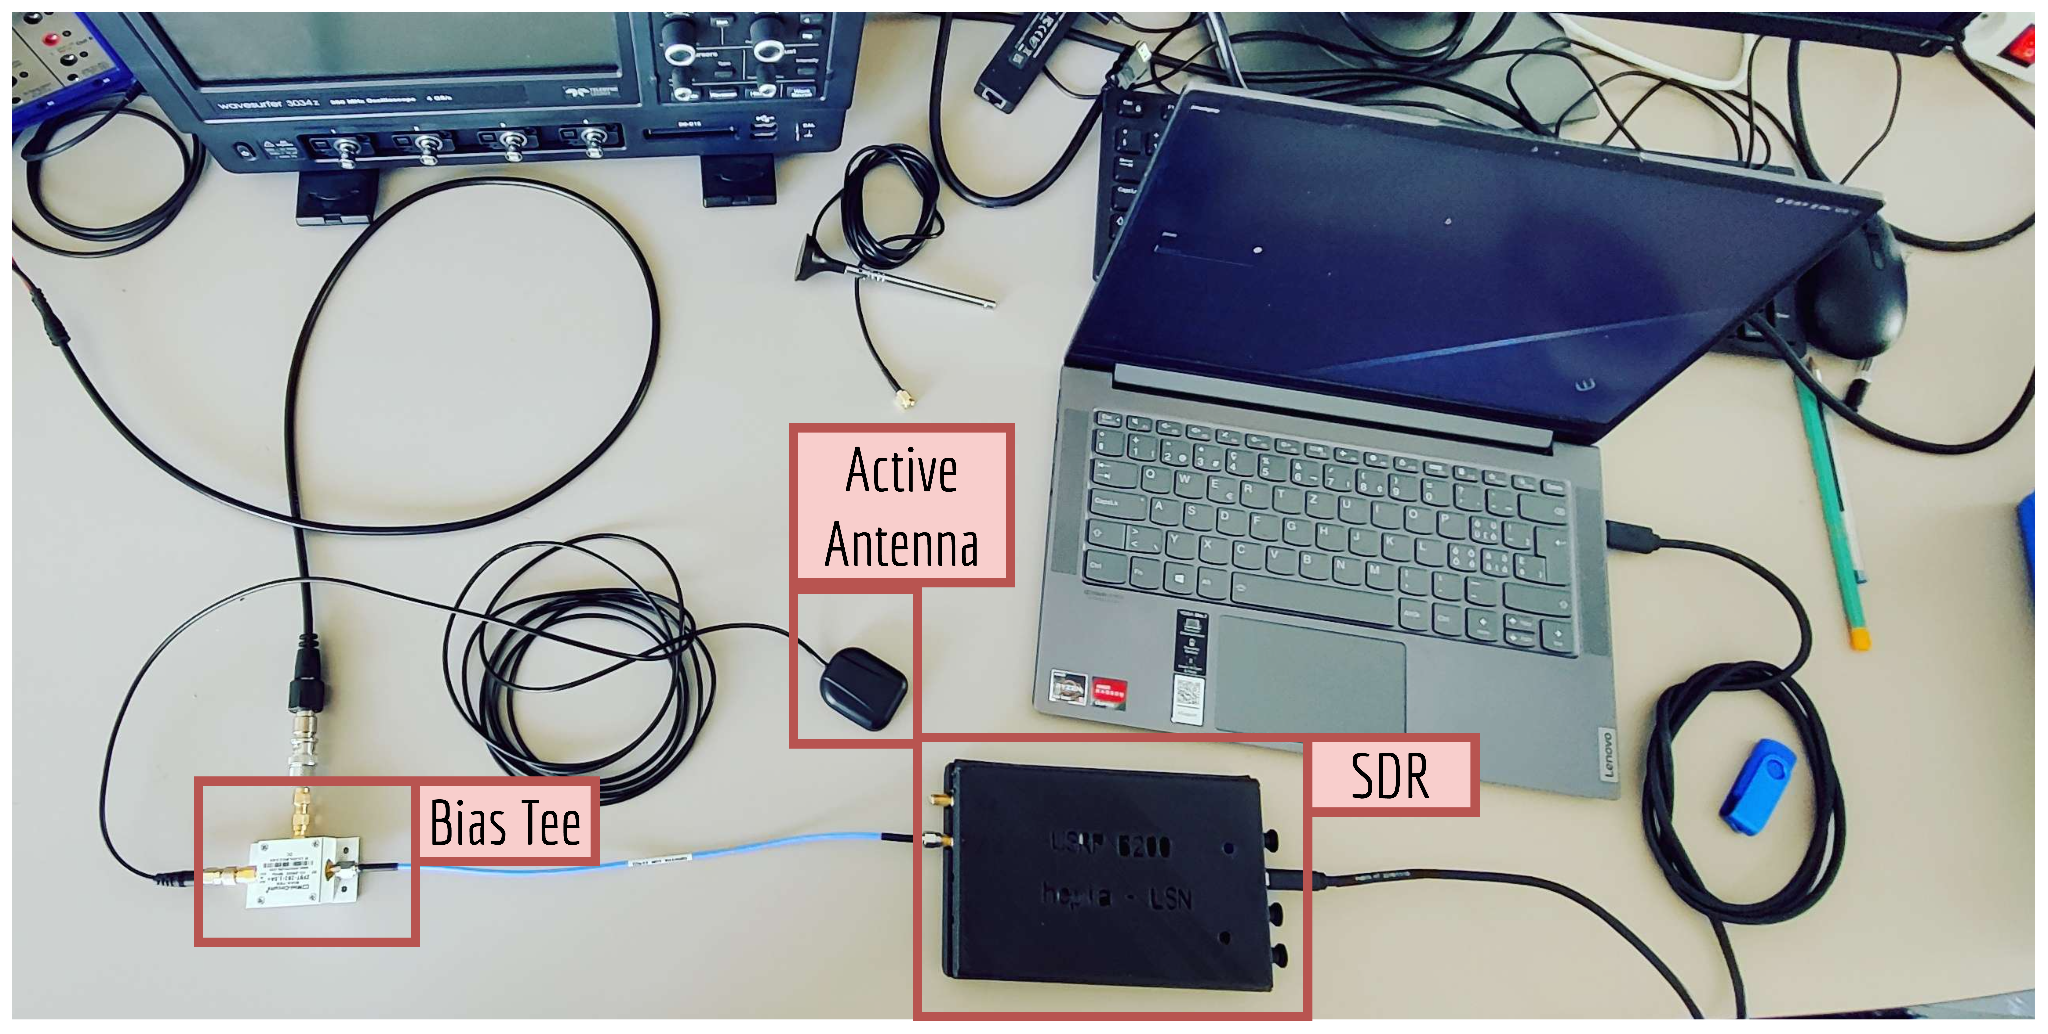
\includegraphics[width=1\linewidth]{first_setup.png}
	\caption[First experiment setup]{First experiment setup with active antenna Source: Made by Jonas Stirnemann}
	\label{fig:first_setup}
\end{figure}


\subsection{Position fix with raw data}
Here is a schematics of the GNU radio flowgraph used to record the raw data:

\begin{figure}[H]
	\centering
	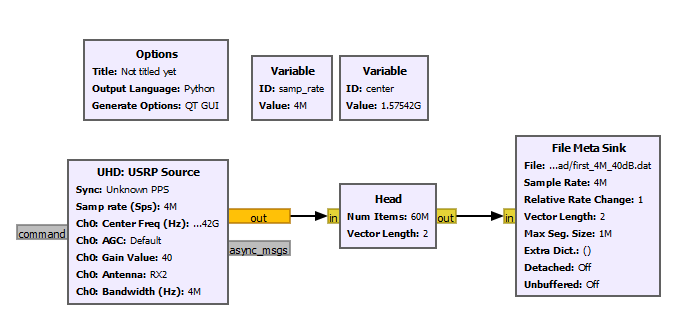
\includegraphics[width=1\linewidth]{gnu_radio.png}
	\caption[Gnu radio schematics raw data]{Gnu radio schematics for recording raw data Source: Made by Jonas Stirnemann}
	\label{fig:gnu_radio}
\end{figure}

After recording some raw data into a file for 5 minutes with the antenna at the window with a relativly correct line of sight of the sky, and after setting everything like it's shown at \footnote{\url{https://gnss-sdr.org/my-first-fix/}}. I tried to get a position fix with GNSS SDR, but I couldn't get a fix. I tried to change the settings, i tried changing the data format but i could not get the fix.

\begin{figure}[H]
	\centering
	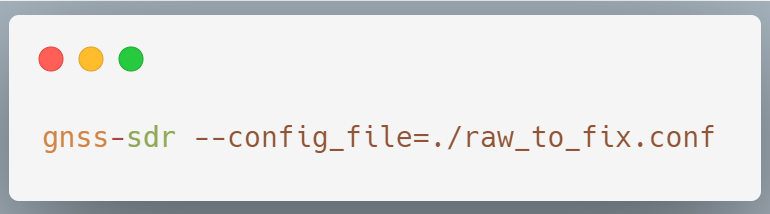
\includegraphics[width=0.7\linewidth]{raw_to_fix.png}
	\caption[Start GNSS SDR]{Start GNSS SDR to get a fix from raw data Source: Made by Jonas Stirnemann}
	\label{fig:start_raw}
\end{figure}

\subsection{Position fix with sdr as direct front end}

Since i could not get a fix with the raw data, i tried to get a fix directly with the USRP B200 as a frontend. The GNSS SDR software provides a way to configure the USRP as a frontend and get a fix directly from the SDR (Configuration in appendix).

After this configuration, I could get a fix with the USRP B200 as a frontend, when finishing the fix, the software saves some files formatted for Google Maps or similar software. So i could check what position fix i had gotten. We can observe the path of the read position in red and the actual position marked as putple dot, even though the accuracy is not our purpose here, we can see that the position goes as far as a 100 meters from the actual position.

\begin{figure}[H]
	\centering
	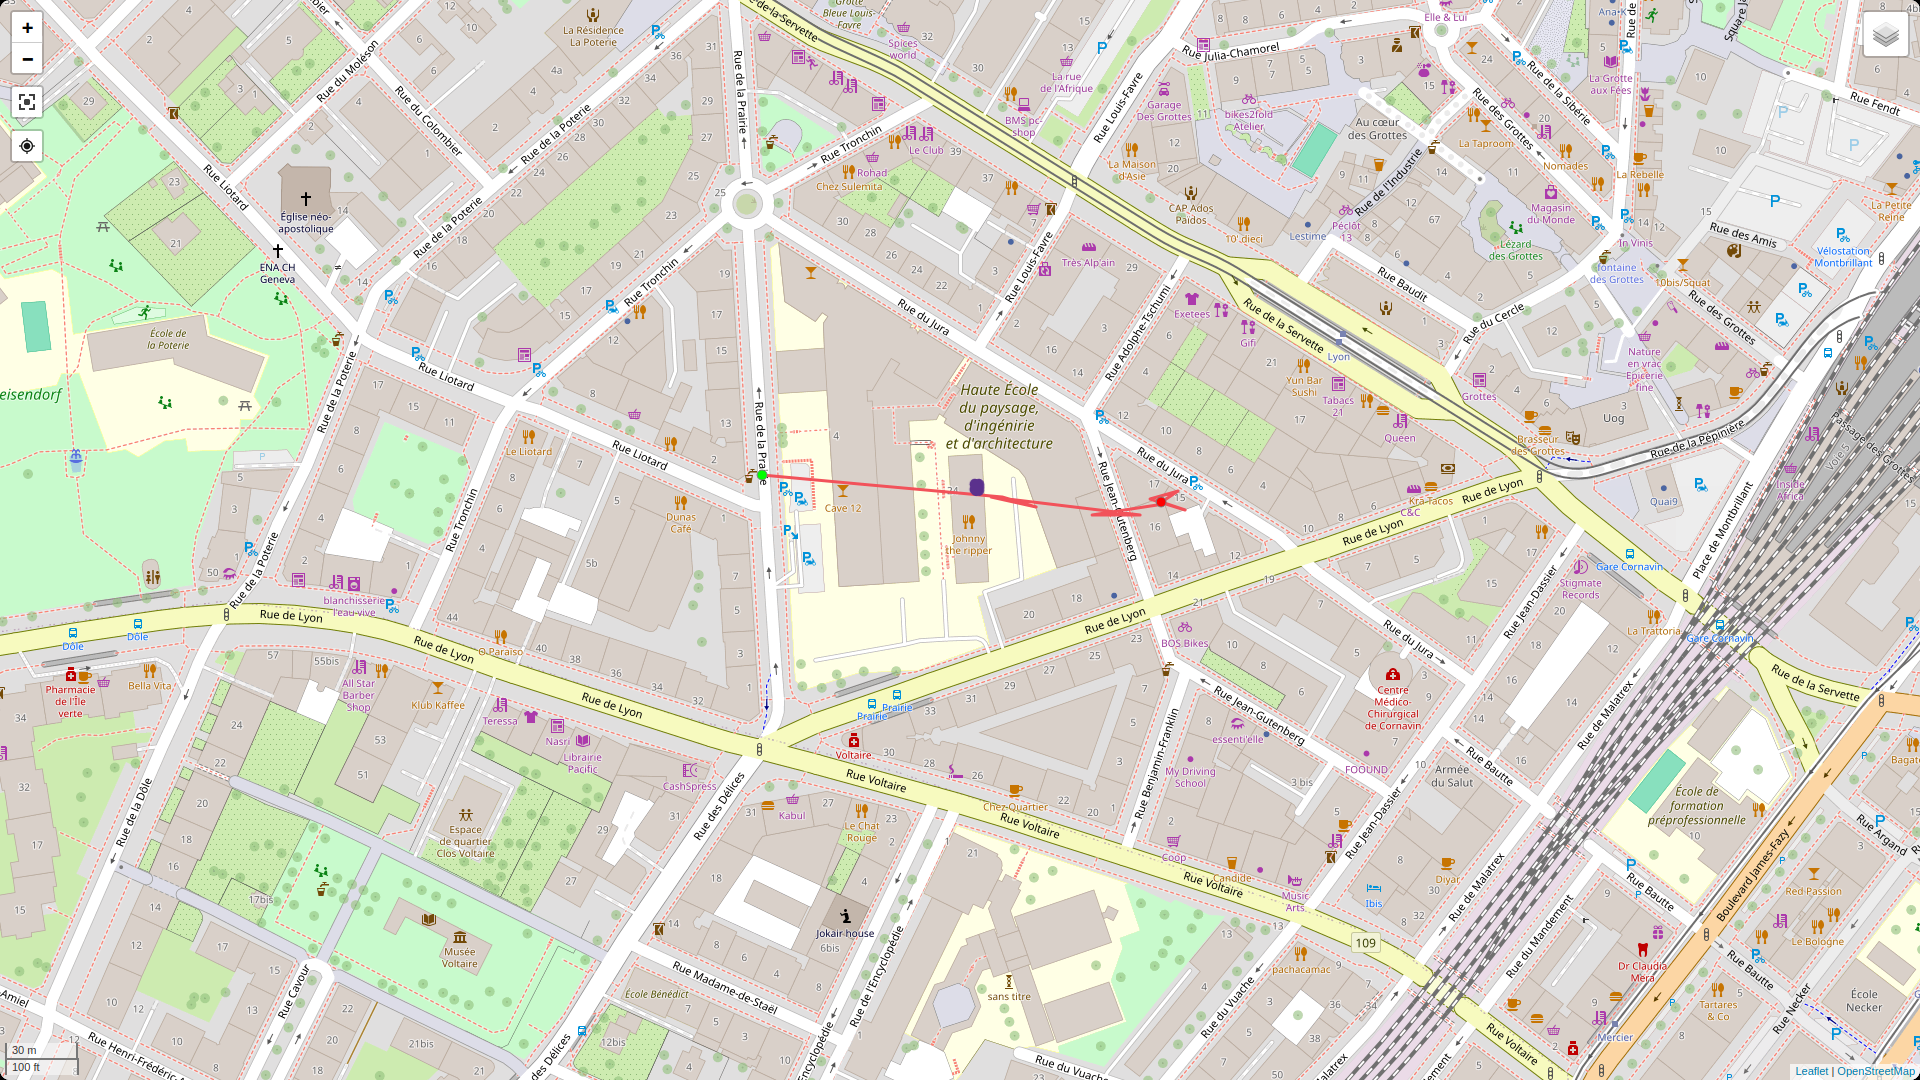
\includegraphics[width=1\linewidth]{gps_view_first_fix.png}
	\caption[First position fix GNSS SDR]{First position fix GNSS SDR Source: Made by Jonas Stirnemann}
	\label{fig:first_fix}
\end{figure}


\section{Receiving position with commercial GPS receiver}

In this second experiment, we'll try to read the position from the commercial GPS receiver with a simple python script reading NMEA data. We'll setup the passive antenna onto the commercial receiver. The receiver has to be externally powered (3.3V by a bench power supply) and is connected via a USB to serial adapter to the computer. The antenna has been placed at the window with a relativly correct line of sight of the sky with a lenght of around 19 cm (according to wavelength of the GPS signal).

\begin{figure}[H]
	\centering
	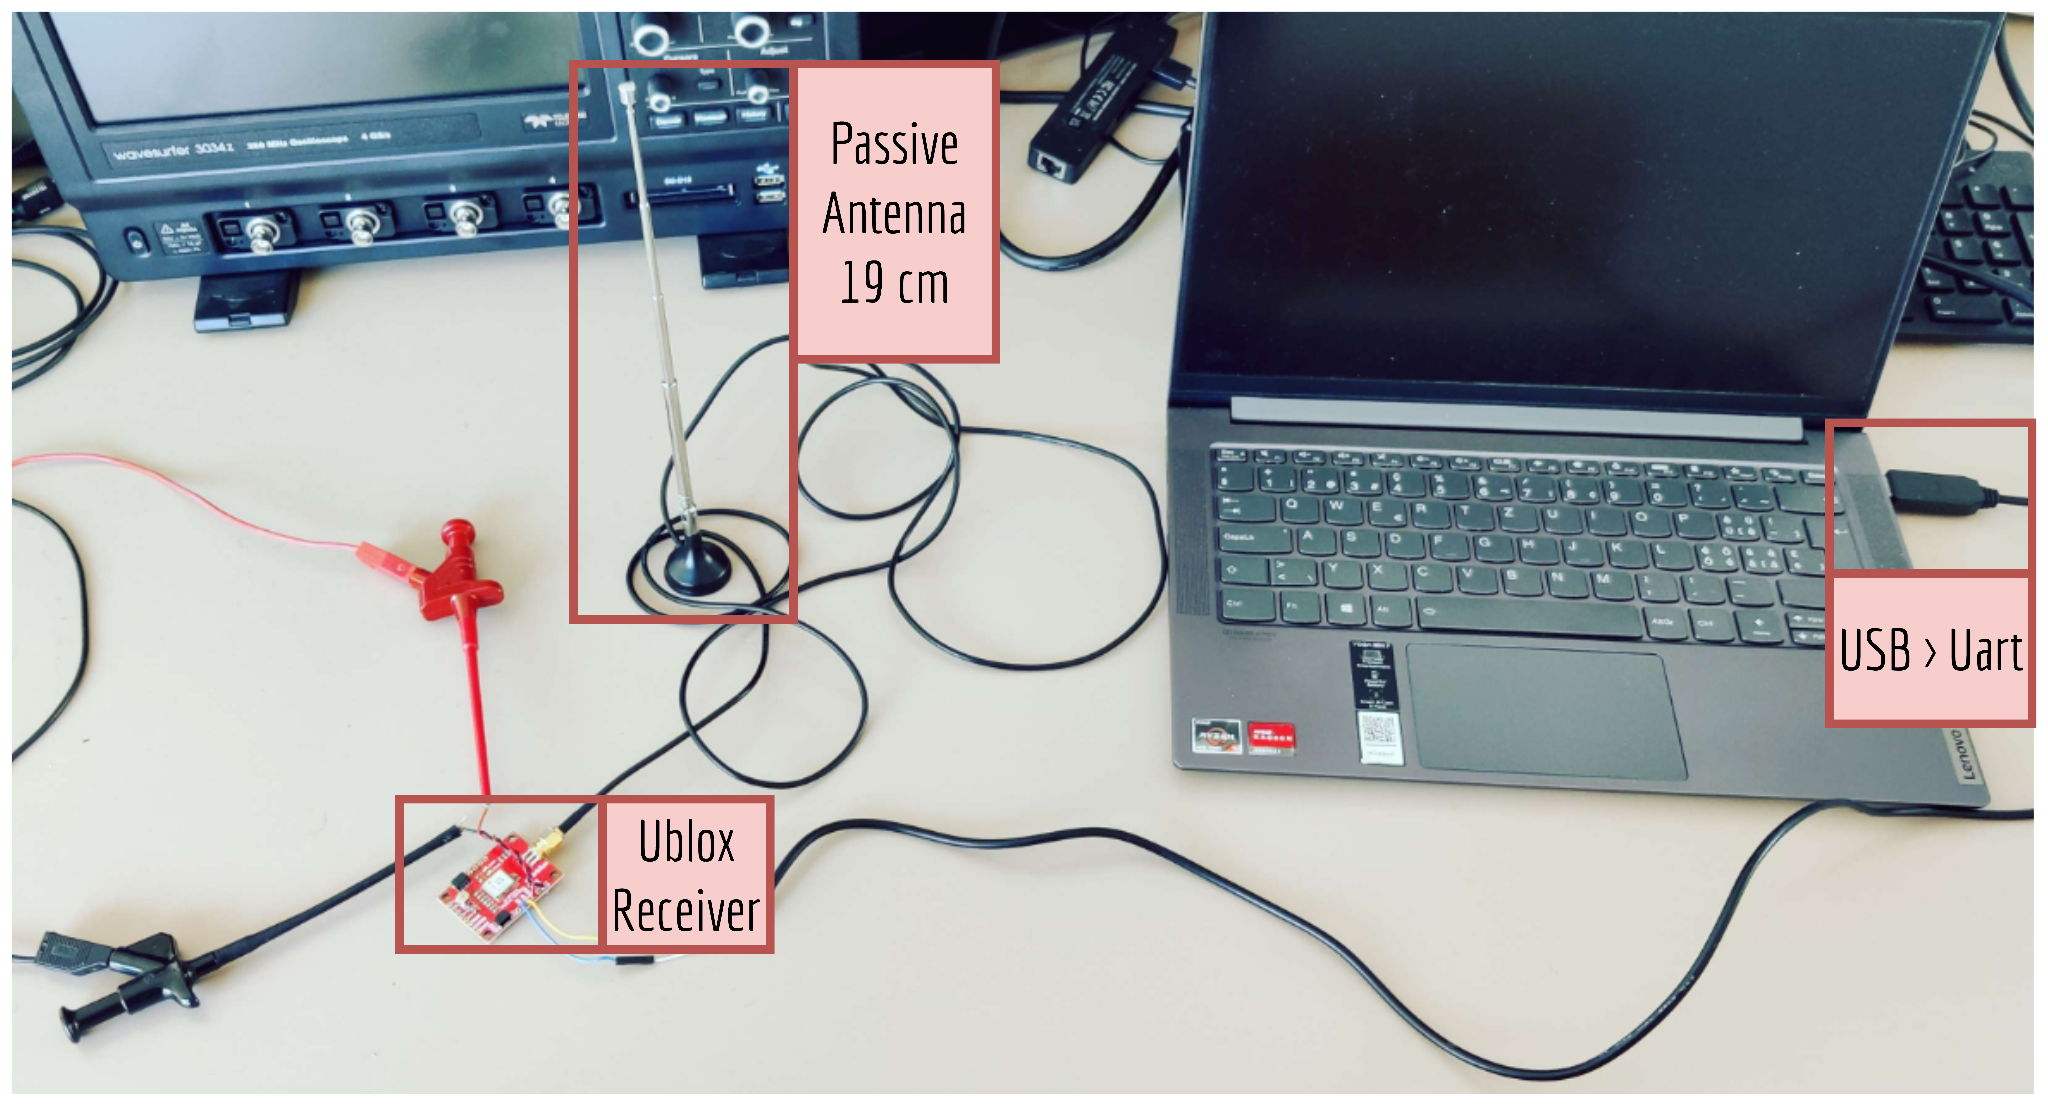
\includegraphics[width=1\linewidth]{second_setup.png}
	\caption[Second Experimentation setup]{Second Experimentation setup with passive antenna Source: Made by Jonas Stirnemann}
	\label{fig:second_setup}
\end{figure}

\subsection{NMEA data format}

The NMEA data format is a standard for GPS data, it is a set of sentences that are sent by the GPS receiver to the computer. The most important sentences are the GGA, RMC and GSA. The GGA sentence contains the position fix, the RMC sentence contains the recommended minimum data for GPS, and the GSA sentence contains the satellite data. The GGA sentence is the most important for us, it contains the latitude and longitude of the receiver.

I used a simple python library called pynmea2 \footcite{noauthor_nmea_2024} to read the NMEA data from the serial port and extract the GGA sentence. The received positions are then renderer in an HTML Open Street Map where we can observe the positions.

\begin{figure}[H]
	\centering
	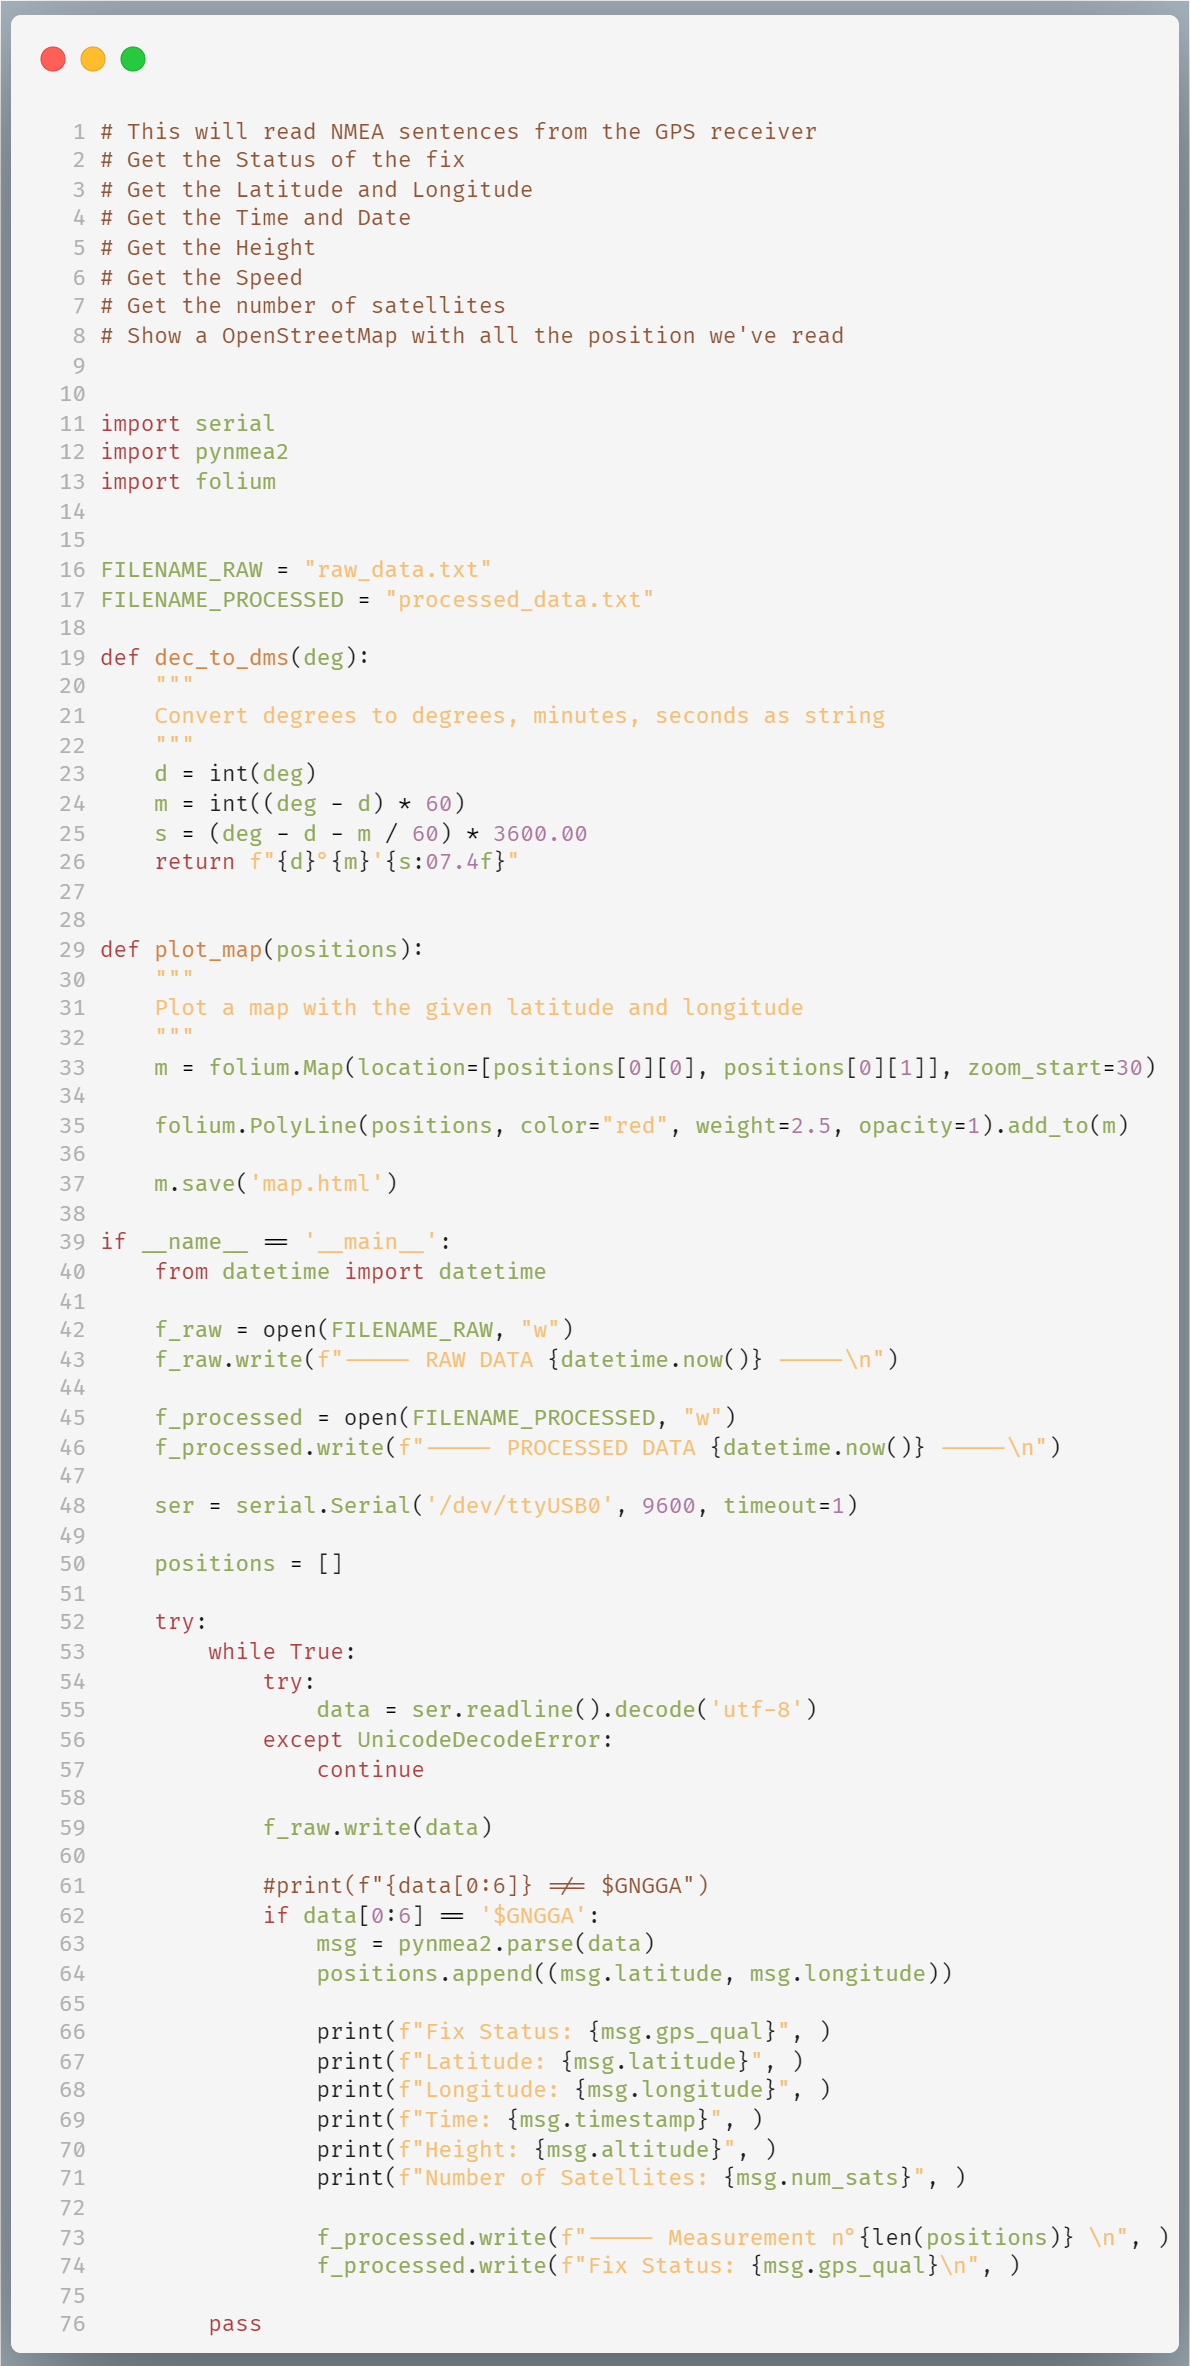
\includegraphics[width=0.7\linewidth]{nmea_code.png}
	\caption[NMEA python script]{NMEA python script reading positions  Source: Made by Jonas Stirnemann}
	\label{fig:nmea_code}
\end{figure}


\begin{figure}[H]
	\centering
	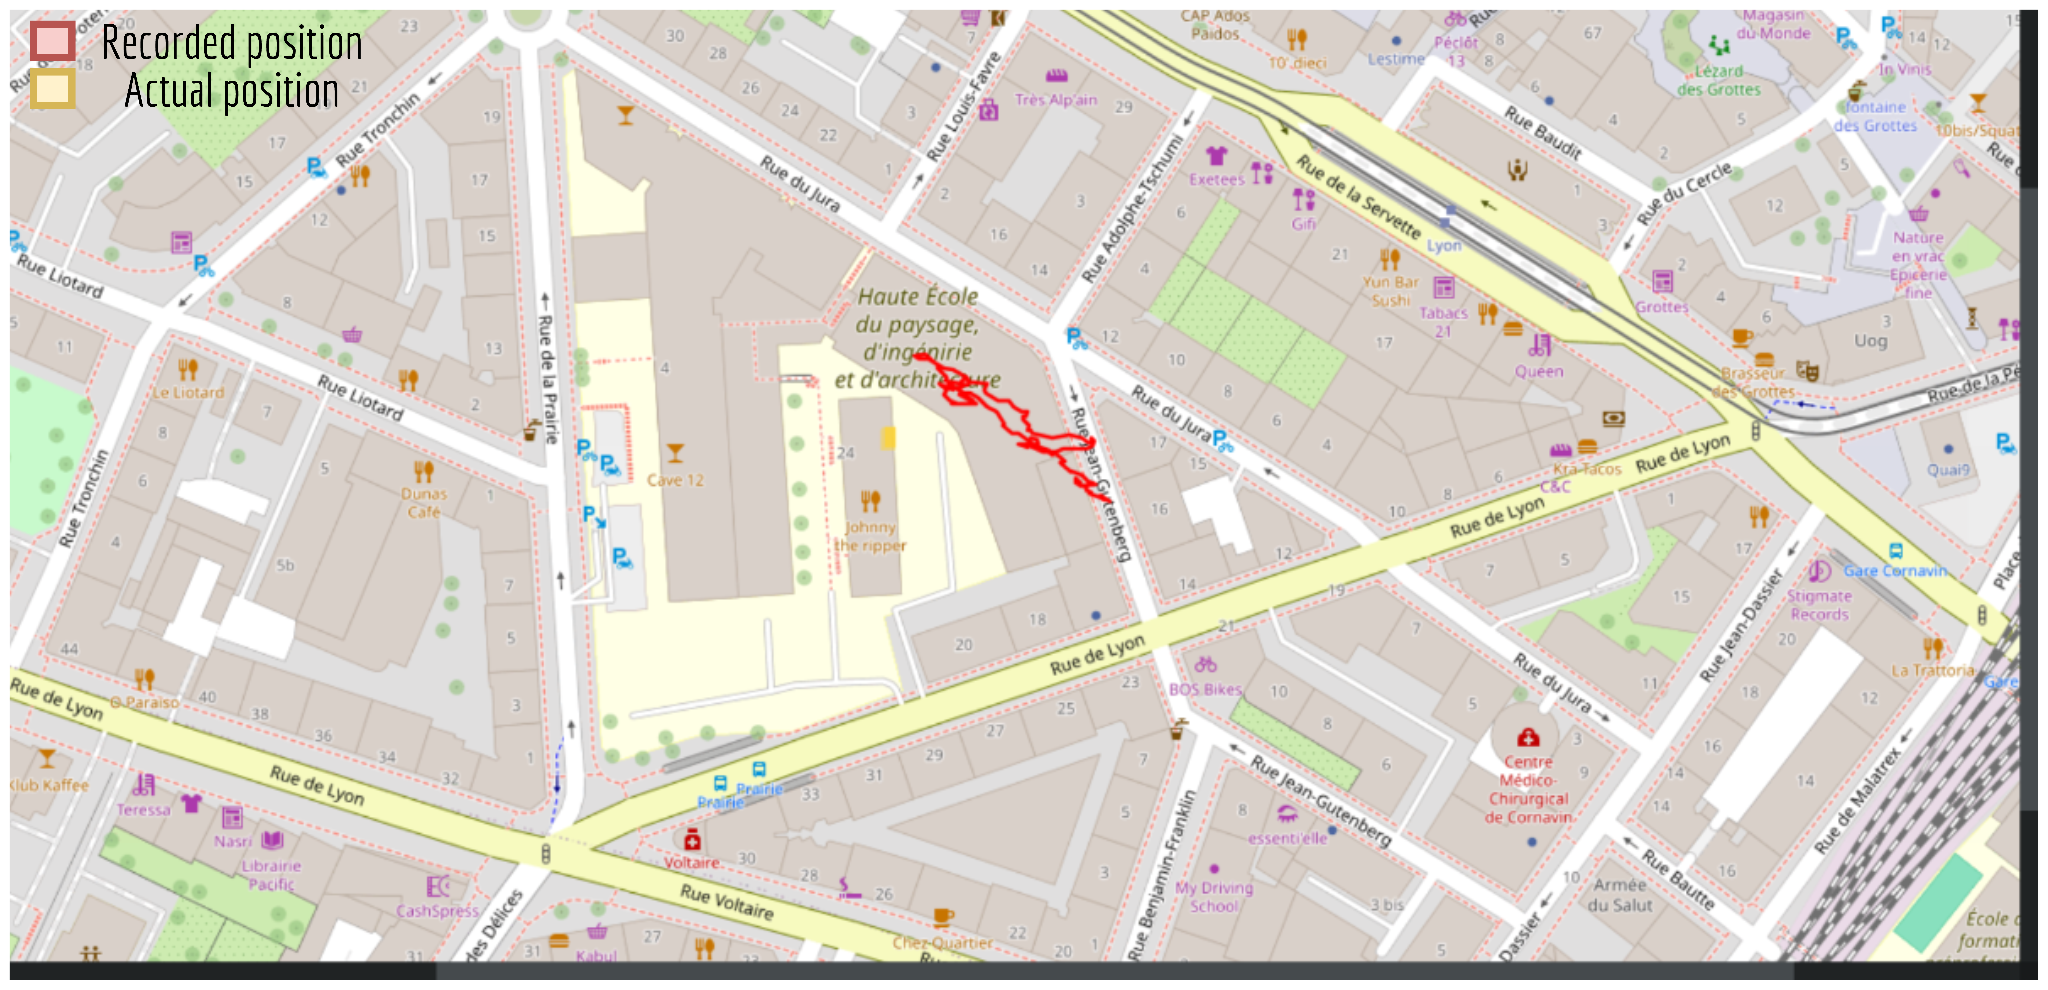
\includegraphics[width=0.7\linewidth]{gps_view_second_fix.png}
	\caption[Second experiment map]{Second experiment map With the positions Source: Made by Jonas Stirnemann}
	\label{fig:second_fix}
\end{figure}

We can observe the path of the read position in red and the actual position marked as orange dot, the accuracy looks really good (around 20m), especially considering we used the passive antenna.

\section{Spoofing GPS position}

Now that we can easily read position from the commercial GPS receiver, we can try to spoof the position with the Multi SDR GPS simulator \footcite{mictronics_mictronicsmulti-sdr-gps-sim_2024}. This software allows us to generate a GPS signal and send it to the USRP B200. We can then send a fake position to the commercial GPS receiver.

\subsection{Battery issue}

I've tried spoofing multiple times but could not get a consistant fix with different spoofed position. It looked like the first time worked but when i changed the spoofed position, the receiver could not get a fix anymore. I've tried to change lots of parameters, i changed the power output from the spoofer but i still could not get a fix.

After some time, i realized that the battery of the commercial GPS receiver was allowing it to store the last ephemeries and almanac data for quicker fix when turned on. But this meant that the receiver would be confused if a completly different position was sent to it. So i decided to remove the battery from the receiver board and it worked every time!

The battery is marked with a purple square, you have to pop it out of the PCB with a knife, scalpel or a screwdriver.

\begin{figure}[H]
	\centering
	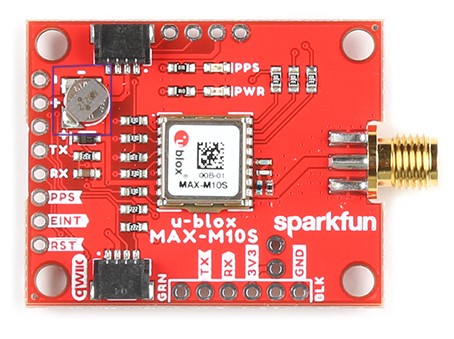
\includegraphics[width=0.7\linewidth]{gps_dev_battery.jpg}
	\caption[GPS receiver dev board battery]{GPS receiver dev board battery marked for removal Source: Made by Jonas Stirnemann}
	\label{fig:battery}
\end{figure}

\subsection{Spoofing position}

In order to setup the spoofing, we have to download the current day almanac data from NASA \footnote{\url{https://cddis.nasa.gov/archive/gnss/data/daily/}}. Then we have to get Multi SDR GPS simulator and start a spoof scenario with the usrp B200 as a frontend.

For example we chose the Toulouse Museum as a spoofed position, the coordinates are : (43.594198064081695, 1.4493044146176086).

\begin{figure}[H]
	\centering
	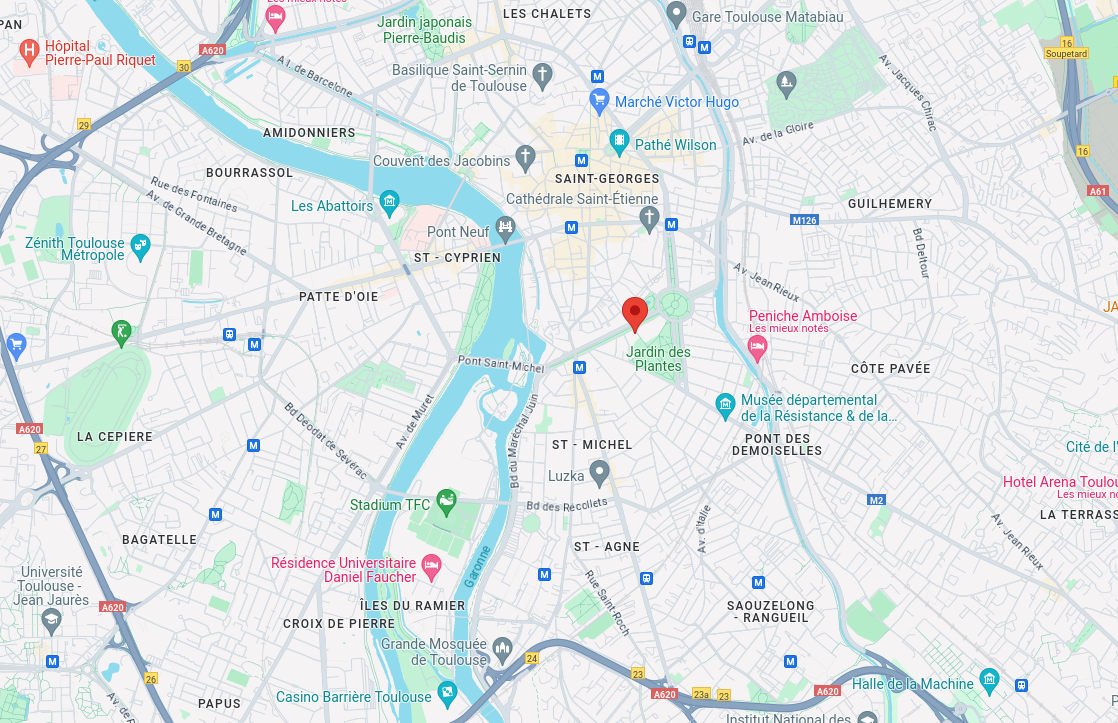
\includegraphics[width=1\linewidth]{real_musee.png}
	\caption[Real Toulouse Museum position]{Real Toulouse Museum position Source: Made by Jonas Stirnemann}
	\label{fig:toulouse_real}
\end{figure}

\begin{figure}[H]
	\centering
	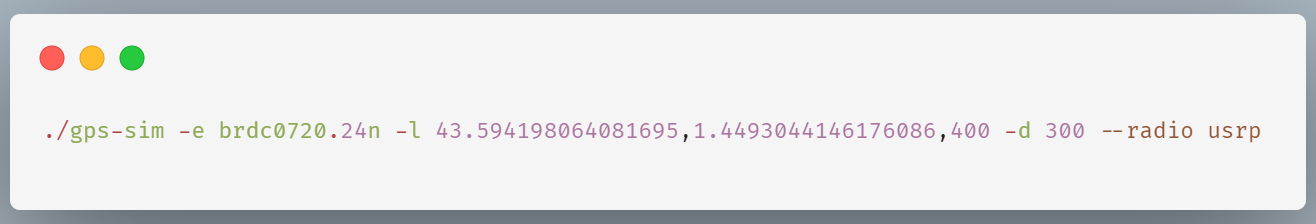
\includegraphics[width=0.7\linewidth]{musee_spoof_code.png}
	\caption[Command to start the spoofing]{Command to start the spoofing Source: Made by Jonas Stirnemann}
	\label{fig:code_start_spoofing}
\end{figure}


Now we can read the position from the commercial GPS receiver and see that the position is spoofed to the Toulouse Museum. After some time, WE GOT A FIX !

\begin{figure}[H]
	\centering
	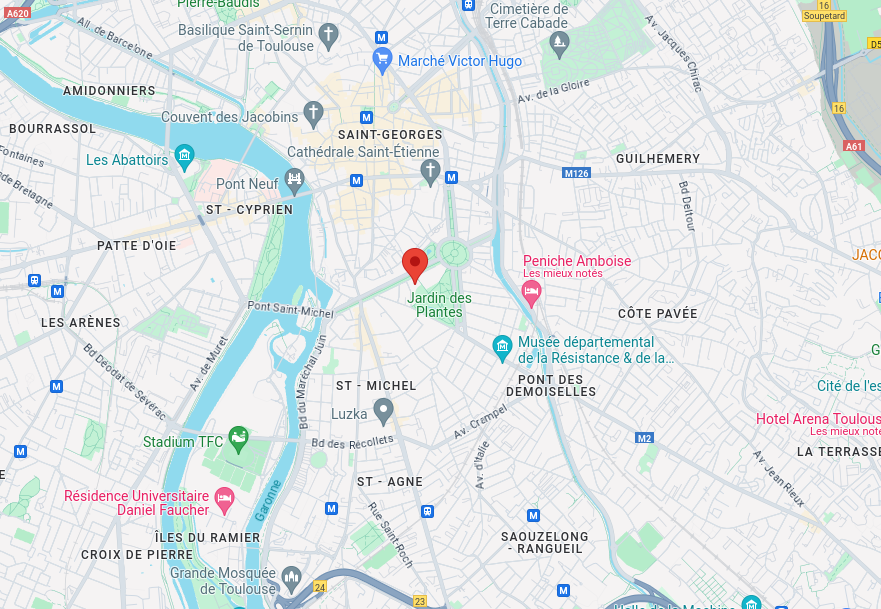
\includegraphics[width=1\linewidth]{spoof_musee.png}
	\caption[Spoofed Toulouse Museum position]{Spoofed Toulouse Museum position Source: Made by Jonas Stirnemann}
	\label{fig:toulouse_spoofed}
\end{figure}


We tried the same with a Viking museum in Oslo, Norway, the coordinates are : (59.90771024065185, 10.683988972697675).

\begin{figure}[H]
	\centering
	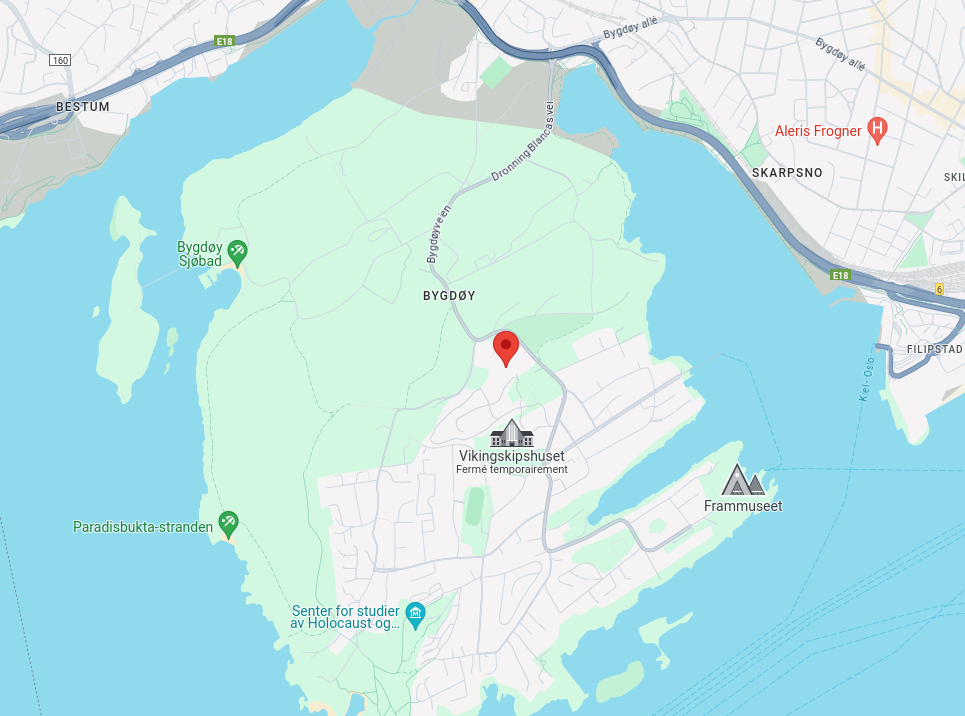
\includegraphics[width=1\linewidth]{real_musee_viking.png}
	\caption[Real Oslo Vikings museum Museum position]{Real Oslo Vikings museum Museum position Source: Made by Jonas Stirnemann}
	\label{fig:viking_real}
\end{figure}

Which then got us a spoofed position really close to the real one.

\begin{figure}[H]
	\centering
	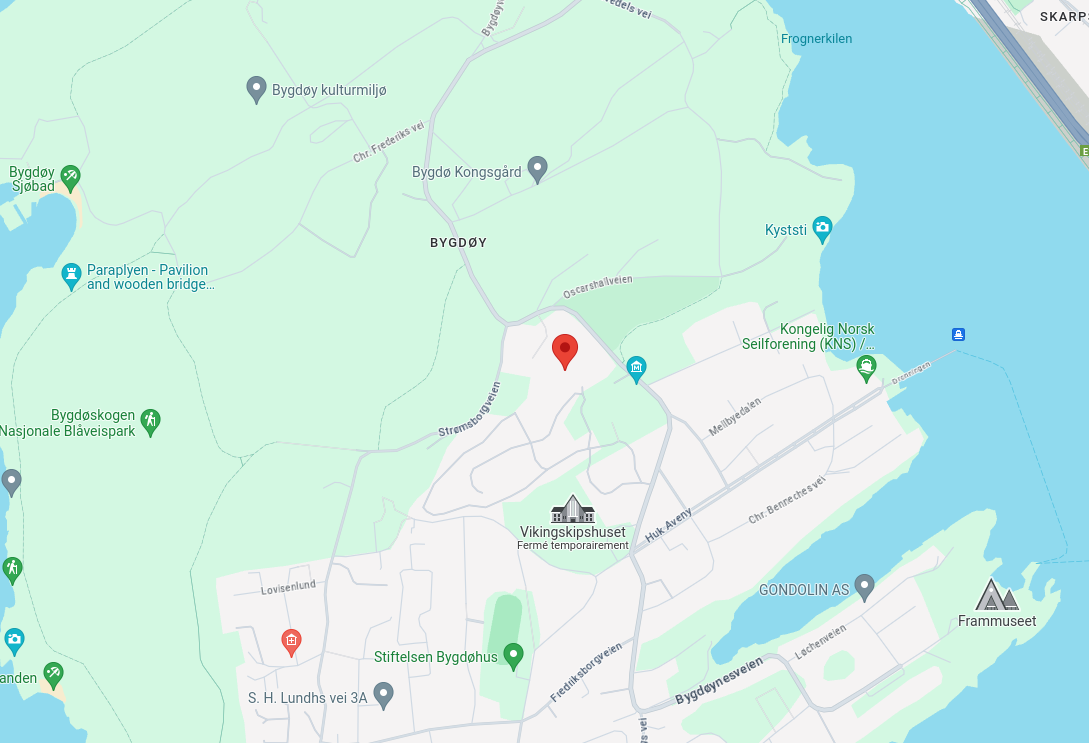
\includegraphics[width=1\linewidth]{spoof_musee_viking.png}
	\caption[Spoofed Oslo Vikings museum Museum position]{Spoofed Oslo Vikings museum Museum position Source: Made by Jonas Stirnemann}
	\label{fig:viking_spoof}
\end{figure}


